\chapter{Introduction}

\emph{Status: Draft. Last Updated 10/8}

A \emph{recommender system} is a software which suggests useful items to a user usually on a website. A user is typically assisted in their search process on the website to find the right item. Recommender systems are able to personalise so that they try to suggest only items relevant for the given user. In order to do this recommender systems rely on multiple techniques, notably \emph{collaborative filtering} and \emph{content-based filtering}.

Recommender systems are usually tightly coupled to the domain and system architecture. Bespoke recommender systems may be very dependent on the system's data model as well as technical constraints such as programming languages. The adaption of recommender systems require knowledge and expertise in both domain and recommender systems. The effort would add more complexity and dependencies to systems, which are probably complex themselves, making change very expensive and time consuming. Being tightly coupled, a recommender implementation is very likely to be incompatible for another use case.

This project aimed to develop and evaluate approaches to unscramble this complexity by abstraction so that domain and recommender systems are independent and insular from each other. Second, the integration of both is to be simplified and eased. Third, the re-usability and interoperability of various recommender systems is to be empowered. Finally, this project is to allow the unconstrained utilisation of the most appropriate technologies for the individual use case.

\section{Background Research}

\emph{Status: Draft. Last Updated 10/8}

\citet{ricci11} write that traditional recommendations can be observed in various scenarios, such as a peer's recommendation when buying a book or reviews when choosing a movie. The authority of the recommender has an important role in the acceptance of the recommendation. A renowned film critic may appear more credible than a random colleague. When it comes to car parts, a mechanist may be a good candidate to ask.

With the growth of the Internet, the amount of information available on the Web increased rapidly. Especially, major e-commerce Web sites were extending their range of products and services. Although a wider and varied range of items is initially good for the user, users found it more and more difficult to find the appropriate items or make the right choices. Web sites have deployed different type of solutions -- such as search engines and more user friendly interfaces -- to cope with this problem.

Another approach are recommender systems which basically provide a bespoke collection of items with the intention to highlight relevant items to a user. Depending on the recommendation technique used, various data sources are taken into account like the user's context or previous interactions. Most recommender systems concentrate on guiding the user towards novel, unexperienced items \cite{herlocker04}.

\subsection{Techniques}

\emph{Status: Draft. Last Updated 10/8}

In the course of development different techniques to compute recommendations emerged. Fundamentally, techniques are classified by the information sources they use. The sources of personalised recommendations are typically user-item interactions (\emph{collaborative filtering}), item features (\emph{content-based filtering}), user features (\emph{demographic filtering}) as well as knowledge about the user and item (\emph{knowledge-based filtering}). Amongst those, the following were implemented in this project:

\subsubsection{Collaborative Filtering}
\label{intro-bg-tech-collaborative}

\emph{Status: Draft. Last Updated 10/8}

\begin{figure}[ht]
    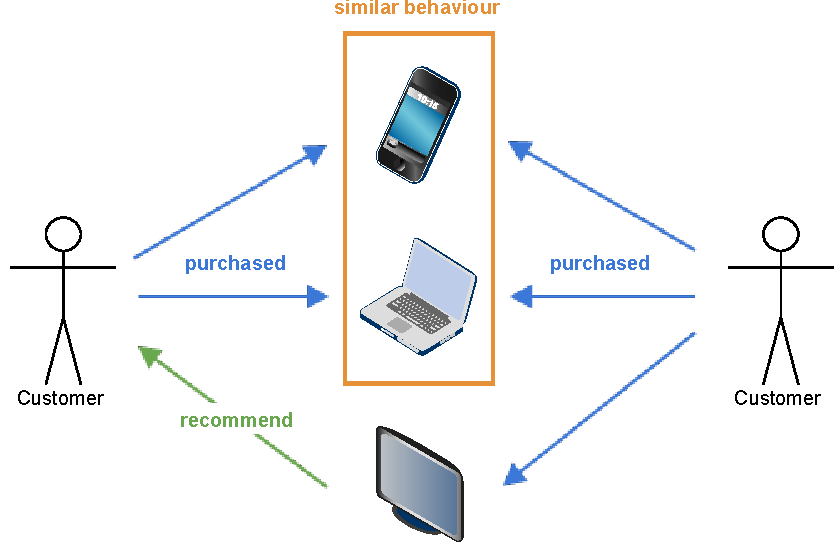
\includegraphics[width=0.7\textwidth,center]{intro/background/collaborative.pdf}
    \caption{Collaborative Filtering}
    \label{fig:collaborative}
\end{figure}

This technique recommends items other users with similar preferences have shown a positive expression e.g. \emph{liked} or \emph{purchased}. In order to do this, the recommender system needs to observe users' behaviours and interactions. Based on these learnings, it will then look up other users with similar behaviour patterns and build recommendations from their preferences -- preferably items which the active user has not experienced yet.

The major advantage of the collaborative filtering approach is that the recommender system does not require any knowledge about the items itself.

Figure \ref{fig:collaborative} illustrates a scenario where the active customer has purchased several items in the past. The recommender system understands that the active customer is similar to another as both have purchased the phone and the laptop. Then, the system computes items the similar customer purchased but the active customer has not. It therefore recommends the TV to the active customer.

\subsubsection{Content-Based Filtering}

\emph{Status: Draft. Last Updated 10/8}

\begin{figure}[ht]
    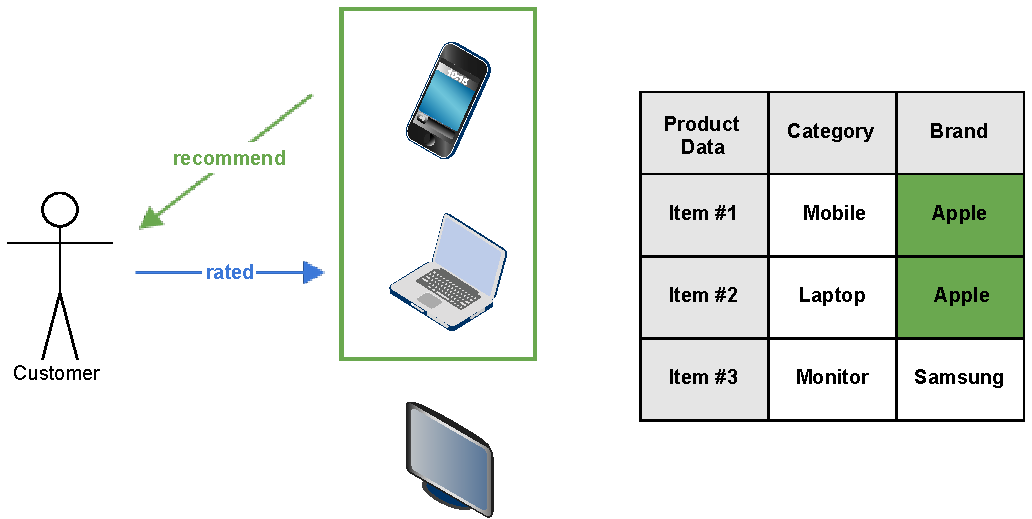
\includegraphics[width=0.7\textwidth,center]{intro/background/contentbased.pdf}
    \caption{Content-Based Filtering}
    \label{fig:contentbased}
\end{figure}

Content-based recommendation methods make use of item features to find similar items. Based on items the user has shown a preference to before -- such as \emph{rated} or \emph{purchased} -- other similar items are looked up based on the item's features. Figure \ref{fig:contentbased} illustrates a customer who has rated an item positively. The recommender system compares the rated item with other items, finds another item which has the same brand and therefore recommends that item.

\subsubsection{Hybrids}
\label{intro-bg-tech-hybrid}

\emph{Status: Draft. Last Updated 10/8}

Hybrid recommender systems make use of two or more individual recommender systems -- hereinafter referred to as components -- to combine aforementioned techniques. One possible motivation of using hybrid systems may be to overcome weaknesses of one approach by combining it with another. However it is also possible to combine systems implementing the same technique but e.g. using different data sources.

There are many possible ways of combining techniques which are outlined in the proposal. In this project, a \emph{weighted} hybrid recommender was implemented which combines the scores of recommender components using a linear formula. A score is a numerical rank attached to items.

\section{Objectives}

\subsection{Abstraction}
\label{intro-objectives-abstraction}

\emph{Status: Draft. Last Updated 10/8}

This objective aims a separation of a system into smaller, loose coupled components and suggests the following criteria:

\begin{description}
    \item[Complexity] Applications such as recommender systems tend to be complex. If not separated, every component adds to the overall complexity making change very difficult, time consuming and expensive. Any change requires knowledge, testing and probably modifications of the whole system.
    \item[Dependency] If a system needs to be modified or even replaced, tightly coupled components become a dependency leading to expensive and tiresome rework.
    \item[Encapsulation] Information hiding is the main motivation behind encapsulation. The more information and implementation is hidden, the looser the coupling becomes. The benefit is that internal changes do not affect other components at all as long as the interfaces remain the same.
    \item[Database Abstraction] Recommender systems with direct access to databases of integrating applications are problematic as these systems are affected by any change of these databases.
    \item[Reusability] Tightly coupled components are difficult to reuse. Reusability is the main driver for multi-purposefulness of this project.
\end{description}

\subsection{Ease of integration}
\label{intro-objectives-easeofintegration}

\emph{Status: Draft. Last Updated 10/8}

The complexity and cost of integration of new systems into existing applications is a major constraint for many projects. This objective covers the ease of integration of applications as well as new recommender techniques. It is measured by the complexity, code footprint, interactions and data volumes of the communication interfaces.

\subsection{Multi-Purpose \& Interoperability}
\label{intro-objectives-multipurpose}

\emph{Status: Draft. Last Updated 22/8}

A \emph{multi-purpose} recommender system is able to cope with different data sources and techniques. Ideally this system is extendable for possible forthcoming, yet unknown requirements.

This multi-purposefulness can be also described in the interoperability between recommender systems. \citet{manouselis07} differentiate between three criteria:

\begin{description}
    \item[Interoperability of the recommendation queries] which allows the same query to be reused. This can be achieved by variable parameters in the query.
    \item[Interoperability of the user and the domain models] which allows the exchange of models and other data among different recommender systems.
    \item[Interoperability of the recommendation results] which empowers recommender systems to reuse the results. This is in particular useful for hybrid recommender systems.
\end{description}

\subsection{Technological Unbiasedness}

\emph{Status: Draft. Last Updated 22/8}

The proposal inarticulately stated another objective to build a mechanism which allows the integration of various recommender techniques to \emph{coexist} and \emph{cooperate}. \emph{Coexistence} refers to supporting various recommender techniques and solutions regardless of technology, language, storage technology and operating system. Furthermore, \emph{cooperation} emphasises the aforementioned interoperability between those recommenders.

\section{Structure of the Report}

\emph{Status: Draft. Last Updated 10/8}

\begin{description}
    \item[Section 3] illustrates the architecture and concepts of various systems of the project.
    \item[Section 4] goes into detail and describes the implementation and technology choices.
    \item[Section 5] reviews the functional and algorithmic correctness of the solutions.
    \item[Section 6] evaluates the project against the project objectives.
    \item[Section 7] reflects on the project outcome and possible future work.
    \item[Appendix A] contains the bibliographical references of the report.
    \item[Appendix B] offers user manuals of the various systems implemented.
    \item[Appendix C] lists the source code written for this project.
\end{description}